\documentclass{beamer}

\usepackage[utf8]{inputenc}
\usepackage[T1]{fontenc}
\usepackage[polish]{babel}
\usepackage{graphicx}
\usepackage{hyperref}

\usetheme{Darmstadt}
\useoutertheme[subsection=false]{miniframes}
\makeatletter
  \beamer@compressfalse
\makeatother

\title{Topologiczna Analiza Danych}
\author{Wojciech Kołowski}
\date{Styczeń 2020}

\begin{document}

\frame{\titlepage}

\addtocontents{toc}{\setcounter{tocdepth}{1}}
\frame{\tableofcontents}

\section{Analiza Danych}

\begin{frame}{Tradycyjne metody analizy danych}
\begin{itemize}
	\item Analiza danych często polega na dopasowaniu do danych jakiegoś uprzednio ustalonego kształtu albo zbadaniu ich struktury.
	\item Regresja liniowa to dopasowanie prostej.
	\item Grupowanie danych to dopasowanie kilku plam o różnym położeniu.
	\item W grupowaniu hierarchicznym dodatkowo jesteśmy zainteresowani grupowaniem grup w grupy wyższego rzędu.
	\item PCA i inne metody redukcji wymiarowości mają na celu dopasowanie danych do jak najmniejszej podprzestrzeni tak, żeby zachować jak najwięcej informacji.
	\item Topologiczna analiza danych (TDA) to technika uogólniająca wszystkie powyższe podejścia za jednym zamachem.
\end{itemize}
\end{frame}

\begin{frame}{Wady tradycyjnych metod analizy danych}
\begin{itemize}
	\item Powyższe podejścia mają wiele różnych wad.
	\item Zasób predefiniowanych kształtów zazwyczaj jest ubogi (zna ktoś algorytm sprawdzający, czy dane nie mają przypadkiem kształtu butelki Kleina?).
	\item Algorytmy grupowania często wymagają zadania liczby grup albo mają inne ograniczenia, np. grupy muszą mieć taki sam kształt albo gęstość.
	\item Grupowanie hierarchiczne może znaleźć hierarchie tam gdzie ich nie ma.
	\item Topologiczna analiza danych spieszy nam na ratunek i poprawia wszystkie te słabości.
\end{itemize}
\end{frame}

\begin{frame}{Kształt danych jako ich podsumowanie}
\begin{itemize}
	\item Topologia to nauka o kształtach, zaś topologiczna analiza danych to dziedzina stosująca topologię do badania kształtu danych.
	\item Zamiast dopasowywać predefiniowany kształt (jak prosta), po prostu znajdujemy faktyczny kształt.
	\item Kształt danych informuje nas o grupach występujących w danych i ich wzajemnych związkach.
	\item Poznanie kształtu danych ujawnia ich prawdziwy wymiar oraz umożliwia ich skompresowanie.
	\item Kształt danych podsumowuje ich najważniejsze właściwości i jest punktem wyjścia do dalszej analizy.
\end{itemize}
\end{frame}

\begin{frame}{Fantastyczne kształty i jak je znaleźć}
\begin{itemize}
	\item Rodzą się zatem różne pytania.
	\item Jak znaleźć kształt danych?
	\item Jakie są w ogóle możliwe kształty?
	\item Co to jest kształt?
	\item ???
	\item Na te pytania odpowie nam geometria, a konkretniej topologia, a konkretniej topologia algebraiczna, a konkretniej metoda zwana z ang. persistent homology.
\end{itemize}
\end{frame}

\section{Topologia}

\begin{frame}{Krótka historia geometrii}
\begin{itemize}
	\item Historycznie topologia wyrosła z analizy matematycznej, ale filozoficznie bliżej jej do geometrii.
	\item Grecka geometria wyrosła z problemów praktycznych (wszak geometria to nic innego jak mierzenie Ziemii), ale szybko wyewoluowała do stanu nieco bardziej Platonicznego.
	\item Grecy myśleli, że wiadomo co to przestrzeń i badali różne rzeczy takie jak punkty, proste, kąty, okręgi, trójkąty etc.
	\item Po odkryciach Łobaczewskiego/Gaussa (geometria nieeuklidesowa), Einsteina (czasoprzestrzeń, do tego zaginana przez masę) i próbach formalnego okiełznania analizy matematycznej okazało się, że jednak nie wiadomo co to przestrzeń.
\end{itemize}
\end{frame}

\begin{frame}{Zgniły geometryczny liberalizm}
\begin{itemize}
	\item Obecnie w geometrii panuje liberalizm -- każdy może mieć taką przestrzeń, jaką sobie zdefiniuje.
	\item Jeżeli chcemy mieć odległość, to potrzebna nam przestrzeń metryczna.
	\item Jeżeli chcemy mieć kąty, to potrzebna nam przestrzeń liniowa z iloczynem skalarnym.
	\item Jeżeli nie chcemy faworyzować żadnych punktów, to potrzebna nam przestrzeń afiniczna -- nie ma tam początku układu współrzędnych.
	\item Jeżeli chcemy rachunek różniczkowy, to potrzebna nam rozmaitość (manifold), czyli przestrzeń, która lokalnie jest euklidesowa, ale globalnie niekoniecznie.
	\item A kto powiedział, że w przestrzeni muszą być jakieś punkty? Patrz: pointless topology.
\end{itemize}
\end{frame}

\begin{frame}{Topologia -- cóż to za zwierzątko?}
\begin{itemize}
	\item Topologia to ten dział geometrii, który ma dość elastyczne podejście do pojęcia przestrzeni -- jeżeli naszą przestrzeń trochę pociągniemy albo pozginamy, dalej jest to ta sama przestrzeń. Nie wolno nam natomiast przestrzeni ciąć ani rwać -- wtedy przestrzeń się zmienia.
	\item Obrazowo: odcinek to prosta, a okrąg to kwadrat. Dla topologa kubek niczym nie różni się od pączka z dziurą, bo kubek można w sposób ciągły przekształcić w pączek. \url{https://en.wikipedia.org/wiki/File:Mug_and_Torus_morph.gif}
	\item Krowa natomiast niczym nie różni się od sfery, co obrazuje poniższy obrazek: \url{https://en.wikipedia.org/wiki/File:Spot_the_cow.gif}
\end{itemize}
\end{frame}

\begin{frame}{Topologia algebraiczna}
\begin{itemize}
	\item W nowoczesnej topologii (i ogólniej w nowoczesnej matematyce) jest taki pomysł, żeby badać obiekty (np. przestrzenie topologiczne) przypisując im jakieś inne obiekty (np. grupy).
	\item Motywacja jest taka, że przypisane obiekty są prostsze w obsłudze, a zawierają wystarczająco informacji dla naszego celu (np. pozwalają odróżniać nieizomorficzne przestrzenie).
	\item Dzięki temu w jednej dziedzinie (topologia) można wykorzystać wiedzę z innej (teoria grup).
	\item Tym właśnie zajmuje się topologia algebraiczna: jak użyć algebry do badania przestrzeni topologicznych.
	\item Znów panuje liberalizm -- nie ma jakiejś jednej nadrzędnej teorii i każdy może sobie wymyślić swoją. Najlepiej mi znaną jest teoria homotopii, ale dla topologicznej analizy danych ważniejsze będą przeróżne teorie homologii.
\end{itemize}
\end{frame}

\begin{frame}{Przykład topologii algebraicznej -- dziury}
\begin{itemize}
	\item Zobaczmy na przykładzie, o co chodzi w topologii algebraicznej.
	\item Jednym z niezmienników, które pozwalają rozróżniać przestrzenie, jest struktura jednowymiarowych dziur w danej przestrzeni.
	\item Dla przykładu, okrąg nie jest tym samym co płaszczyzna, odcinek ani sfera, bo okrąg ma jednowymiarową dziurę, zaś płaszczyzna, odcinek ani sfera nie mają jednowymiarowych dziur.
	\item Co to jest dziura, jak możemy ją opisać i wykryć?
	\item Są różne teorie, między innymi teoria homotopii oraz teoria homologii. Przyjrzyjmy się obu.
	\item Ostrzeżenie: poniższe slajdy dotyczące teorii homotopii są w zasadzie nie na temat, tzn. nie mają związku z topologiczną analizą danych.
\end{itemize}
\end{frame}

\begin{frame}{Teoria homotopii -- intuicja}
\begin{itemize}
	\item Kluczowe jest pojęcie pętli i ich homotopii.
	\item Pętla w punkcie $x$ to ścieżka, która zaczyna się i kończy w punkcie $x$.
	\item Dwie pętle (o początku i końcu w tym samym punkcie) są homotopiczne, jeżeli można w sposób ciągły przekształcić jedną na drugą.
	\item Obrazek (ale dla ścieżek, a nie dla pętli): \url{https://en.wikipedia.org/wiki/File:HomotopySmall.gif}
	\item W każdym punkcie $x$ jest też pętla, którą pójście polega tak na prawdę na staniu w miejscu. Zwie się ona pętla trywialną.
	\item Jeżeli jakaś pętla nie jest homotopiczna z pętlą trywialną, to znaczy, że biegnie dookoła dziury.
	\item Jak to wszystko formalnie opisać?
\end{itemize}
\end{frame}

\section{Homotopia}

\begin{frame}{Teoria homotopii -- grupa podstawowa 1}
\begin{itemize}
	\item Jeżeli mamy przestrzeń $X$ i punkt $x$, to wszystkie pętle w $x$ tworzą grupę (uwaga: przyjmujemy, że pętle są równe, jeżeli są homotopiczne).
	\item Działanie to sklejanie pętli: mając dwie pętle, możemy najpierw pójść jedną, a potem drugą, co w wyniku też daje pętlę.
	\item Element neutralny to pętla trywialna.
	\item Odwrotność pętli to pójście nią w przeciwnym kierunku.
	\item Grupa wszystkich pętli o początku i końcu w punkcie $x$ z działaniem jak powyżej zwie się grupą podstawową, $\pi_1(X, x)$.
	\item Co więcej, każda funkcja ciągła $f: X \to Y$, która zachowuje wyróżniony punkt (czyli $f(x) = y$), daje homomorfizm grup $\tilde{f}: \pi_1(X, x) \to \pi_1(Y, y)$.
\end{itemize}
\end{frame}

\begin{frame}{Teoria homotopii -- grupa podstawowa 2}

\hspace*{-1.05cm}
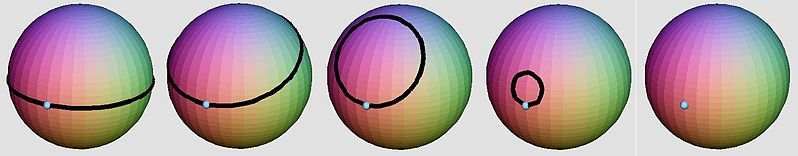
\includegraphics[scale = 0.45]{P1S2.jpg}

Grupa podstawowa sfery $S^2$ jest trywialna, bo każdą pętlę można przekształcić w pętle trywialną, co demonstruje obrazek.

\hspace{1cm}
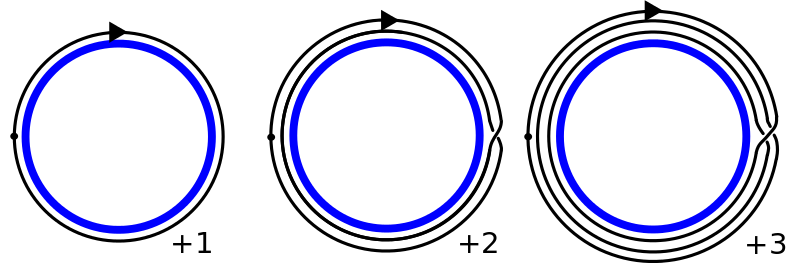
\includegraphics[scale = 0.3]{P1S1.png}

Grupa podstawowa okręgu to $\mathbb{Z}$, bo możemy stać w miejscu ($0$), pójść $k$ razy zgodnie z ruchem wskazówek zegara ($+k$), albo przeciwnie do ruchu wskazówek zegara ($-k$)

\end{frame}

\begin{frame}{Teoria homotopii -- grupa podstawowa 3}
\begin{itemize}
	\item Dla odcinka $[0, 1]$ oraz prostej $\mathbb{R}$, dysku i kwadratu (pełnego w środku) grupa podstawowa jest trywialna, podobnie jak dla sfery.
	\item Stąd wniosek, że okrąg nie jest izomorficzny ze sferą/prostą/odcinkiem/dyskiem/kwadratem etc.
	\item Lista grup podstawowych różnych przestrzeni: \url{http://mathonline.wikidot.com/list-of-fundamental-groups-of-common-spaces}
\end{itemize}
\end{frame}

\begin{frame}{Teoria homotopii -- problemy obliczeniowe}
\begin{itemize}
	\item Teoria homotopii nie jest bez wad.
	\item Wada obliczeniowa jest taka, że wyższe grupy homotopii (czyli grupy opisujące dziury o wymiarze $\geq 1$) trudno jest obliczyć -- znane są algorytmy to robiące, ale w większości ciekawych przypadków nikt nigdy nie doczekał się, aż skończyły pracę.
	\item Wobec powyższego ciężko liczyć na to, że teoria homotopii nada się do analizy danych.
\end{itemize}
\end{frame}

\begin{frame}{Teoria homotopii -- problemy konceptualne}

\vspace{-0.3cm}
\begin{center}
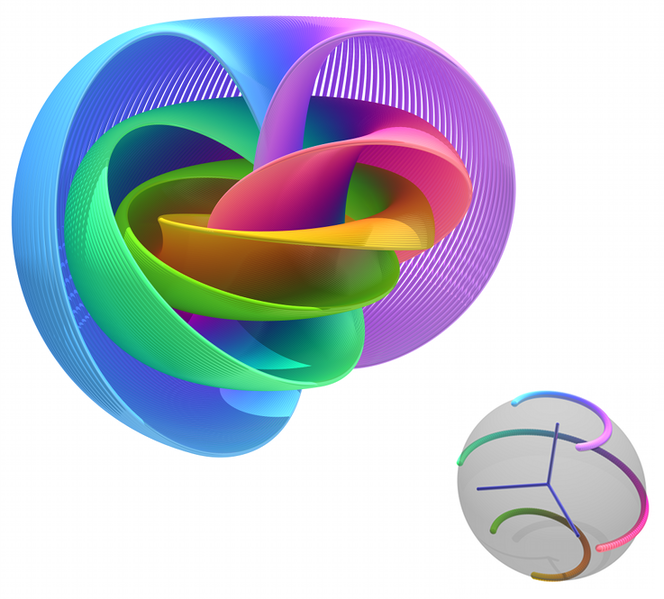
\includegraphics[scale = 0.3]{FibracjaHopfa.png}
\end{center}
\vspace{-0.5cm}

Nieco ciekawsza jest ''wada'' konceptualna: (wyższe) grupy homotopii są bardzo nietrywialne i zaskakujące, np. dwuwymiarowa sfera $S^2$ ma trójwymiarową dziurę, znaną jako fibracja Hopfa.

\end{frame}

\section{Kompleksy}

\begin{frame}{Droga do homologii}
\begin{itemize}
	\item Bardziej przyjaznymi teoriami, zarówno pod względem algorytmicznym, jak i braku trójwymiarowych dziur w dwuwymiarowych obiektach, są przeróżne teorie homologii.
	\item Za chwilę przyjrzymy się czemuś, co z ang. nazywa się simplicial homology, czyli teorii homologii dla simpleksów i kompleksów.
	\item Teoria używana w topologicznej analizie danych zwie się natomiast z ang. persistent homology i zobaczymy ją głównie na obrazkach.
	\item Zanim jednak do tego dojdzie, musimy odpowiedzieć sobie na parę podstawowych pytań.
\end{itemize}
\end{frame}

\begin{frame}{Jak reprezentować przestrzenie w komputerze? 1}
\begin{itemize}
	\item Przestrzenie mogą być skomplikowane.
	\item Mogą mieć nieprzeliczalnie wiele punktów, a komputery mają przecież skończoną pamięć.
	\item Mogą być gładkie i ciągłe, a komputery operują przecież na dyskretnych danych.
	\item Mogą rozciągać się w nieskończoność (zauważ, że to inna właściwość, niż posiadanie nieskończonej ilości punktów).
	\item Przykładem upierdliwej przestrzeni mającej dwie pierwsze właściwości jest torus.
\end{itemize}

\begin{center}
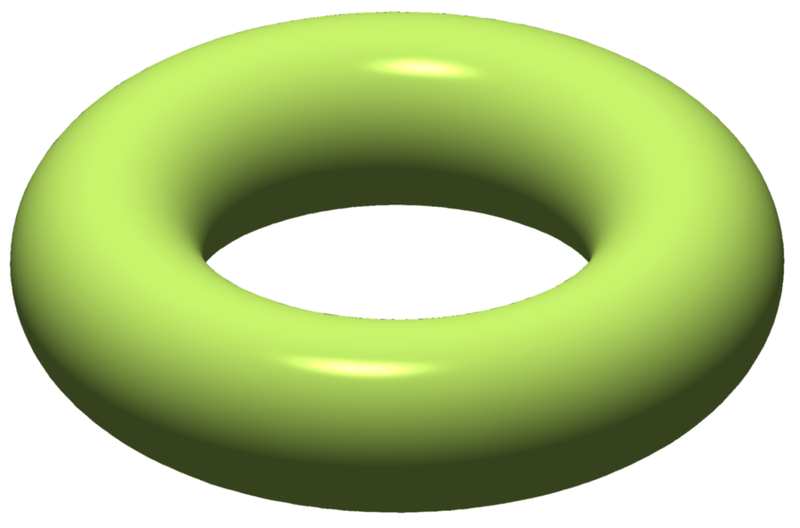
\includegraphics[scale = 1]{Torus.png}
\end{center}

\end{frame}

\begin{frame}{Jak reprezentować przestrzenie w komputerze? 2}
\begin{itemize}
	\item Sytuacja jest podobna jak z liczbami rzeczywistymi. Jak je reprezentować? Nie da się, więc konieczne jest przybliżenie, czyli liczby zmiennoprzecinkowe.
	\item Analogicznie dla przestrzeni: każdą niepatologiczną przestrzeń można przybliżyć za pomocą pewnej ilości prostych figur geometrycznych, jak trójkąty, kwadraty etc. Poetycko zwie się to triangulacją.
\end{itemize}

\begin{center}
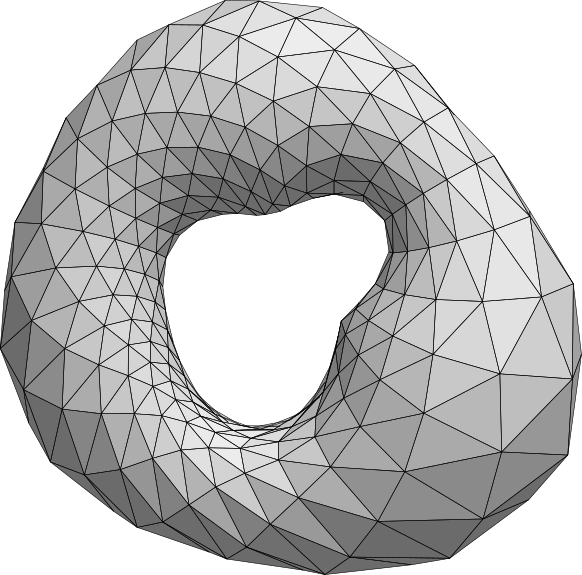
\includegraphics[scale = 0.2]{TriangulacjaTorusa.png}
\end{center}

\end{frame}

\begin{frame}{Simpleksy}

\begin{itemize}
	\item Torus jest dwuwymiarowy, więc do jego triangulacji wystarczą same trójkąty, ale przestrzenie więcej niż dwuwymiarowe wymagają czegoś więcej.
	\item Na ratunek przychodzą nam simpleksy. Simpleks to uogólnienie trójkąta na dowolną liczbę wymiarów.
	\item $0$-simpleks to punkt, $1$-simpleks to odcinek, $2$-simpleks to trójkąt, $3$-simpleks to czworościan, $4$-simpleks to... wyobraźnio do boju.
\end{itemize}

\begin{center}
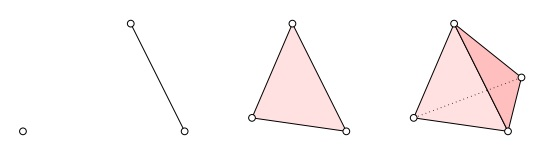
\includegraphics[scale = 0.6]{Simpleksy.jpg}
\end{center}

\end{frame}

\begin{frame}{Kompleksy}
\begin{itemize}
	\item Kompleks (ang. simplicial complex) to byt zrobiony z simpleksów.
	\item Jeżeli $\sigma$ i $\tau$ są simpleksami w kompleksie $C$, to ich przecięcie $\sigma \cap \tau$ też musi być simpleksem w $C$.
	\item Jeżeli $\sigma$ jest simpleksem w kompleksie $C$, zaś $\tau$ jest krawędzią/ścianą (jak to nazwać w wyższym wymiarze?) $\sigma$, to $\tau$ jest simpleksem w $C$.
	\item Formalniej kompleks możemy reprezentować za pomocą rodziny zbiorów, np. $\{\{a\}, \{b\}, \{c\}, \{a, b\}, \{b, c\}, \{a, c\}, \{a, b, c\}, \{d\}, \{a, d\}\}$ to trójkąt z odcinkiem $ad$ przyklejonym do $a$ (sprawdź to).
\end{itemize}
\end{frame}

\begin{frame}{Kompleksy -- przykład}

\begin{center}
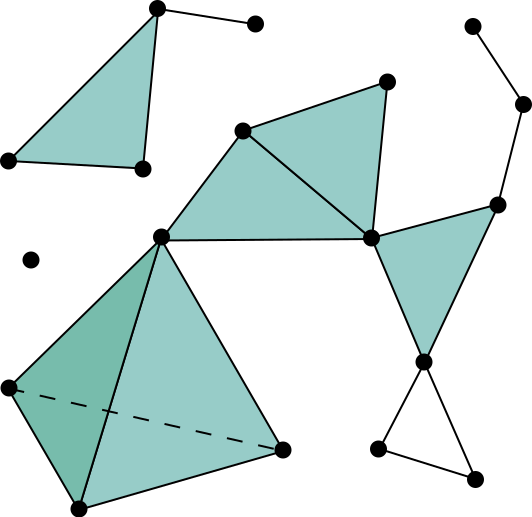
\includegraphics[scale = 0.35]{Kompleks.png}
\end{center}

Ćwiczenie: opisz formalnie (jako zbiór) kompleks z obrazka.

\end{frame}

\begin{frame}{Kompleksy - antyprzykład}
\hspace*{-2cm}
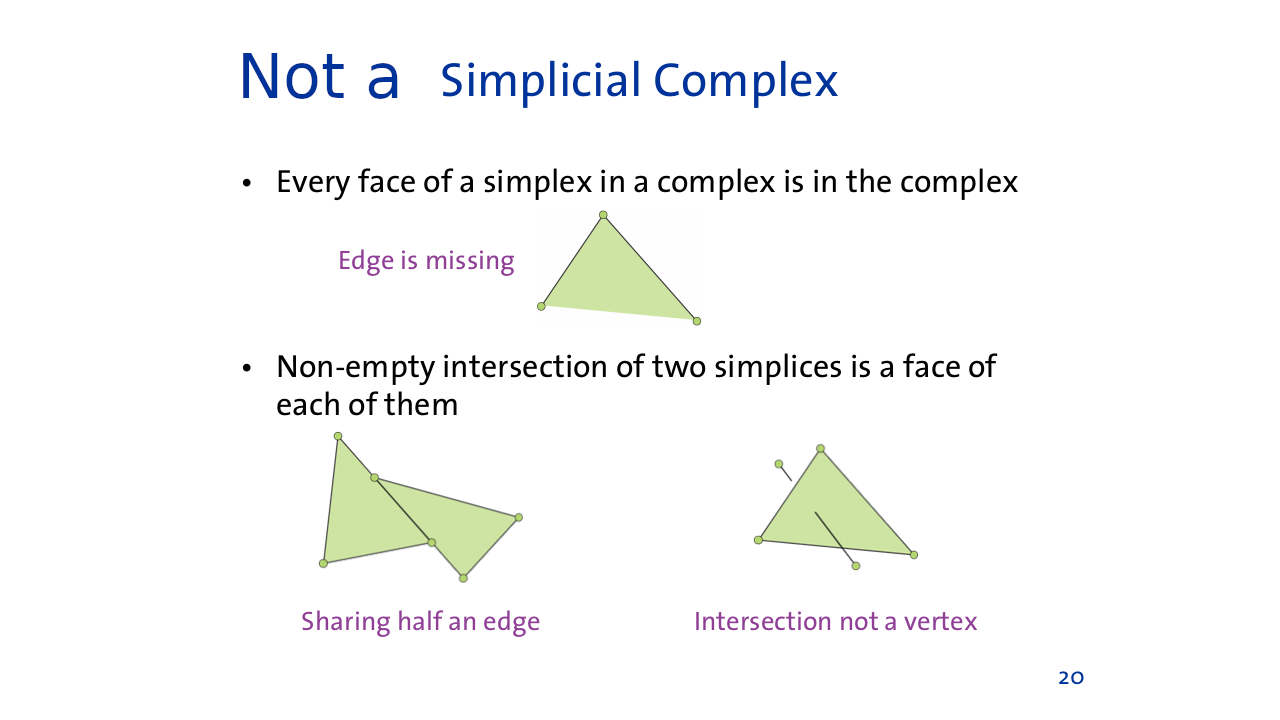
\includegraphics[scale=1.43]{NieKompleks.png}
\end{frame}

\section{Homologia}

\begin{frame}{Teoria dziur, znowu}
\begin{itemize}
	\item Jest intuicyjnie jasne, że trójkąt (pełny w środku) nie zawiera żadnej dziury, ale jego brzeg (czyli trzy odcinki) zawiera dziurę.
	\item Jak sformalizować tę intuicję?
	\item A jak rozszerzyć ją na dziury wyższego wymiaru?
	\item Podstawową rzeczą, jaką można zrobić z dziurą i nie zrobić sobie przy tym krzywdy, to chodzenie dookoła niej.
	\item Oczywiście można też chodzić dookoła rzeczy, które nie są dziurami.
	\item Te dwa podstawowe fakty już niedługo posłużą nam do zdefiniowania grup homologii, ale najpierw kilka niezbędnych definicji.
\end{itemize}
\end{frame}

\begin{frame}{Orientacja 1}

\begin{itemize}
	\item Niech $C$ będzie kompleksem. O każdym simpleksie $\sigma \in C$ możemy myśleć, że ma jakąś orientację.
	\item Zorientowane simpleksy możemy reprezentować za pomocą ciągów wierzchołków.
	\item Dla odcinków orientacja to po prostu kierunek. $ab$ idzie z lewa na prawo, a $ba$ z prawa na lewo.
	\item Dla trójkątów orientacja to wybór definicji dla ''zgodnie z ruchem wskazówek zegara''. $abc$ to zgodnie, zaś $acb$ -- przeciwnie.
\end{itemize}

\begin{center}
	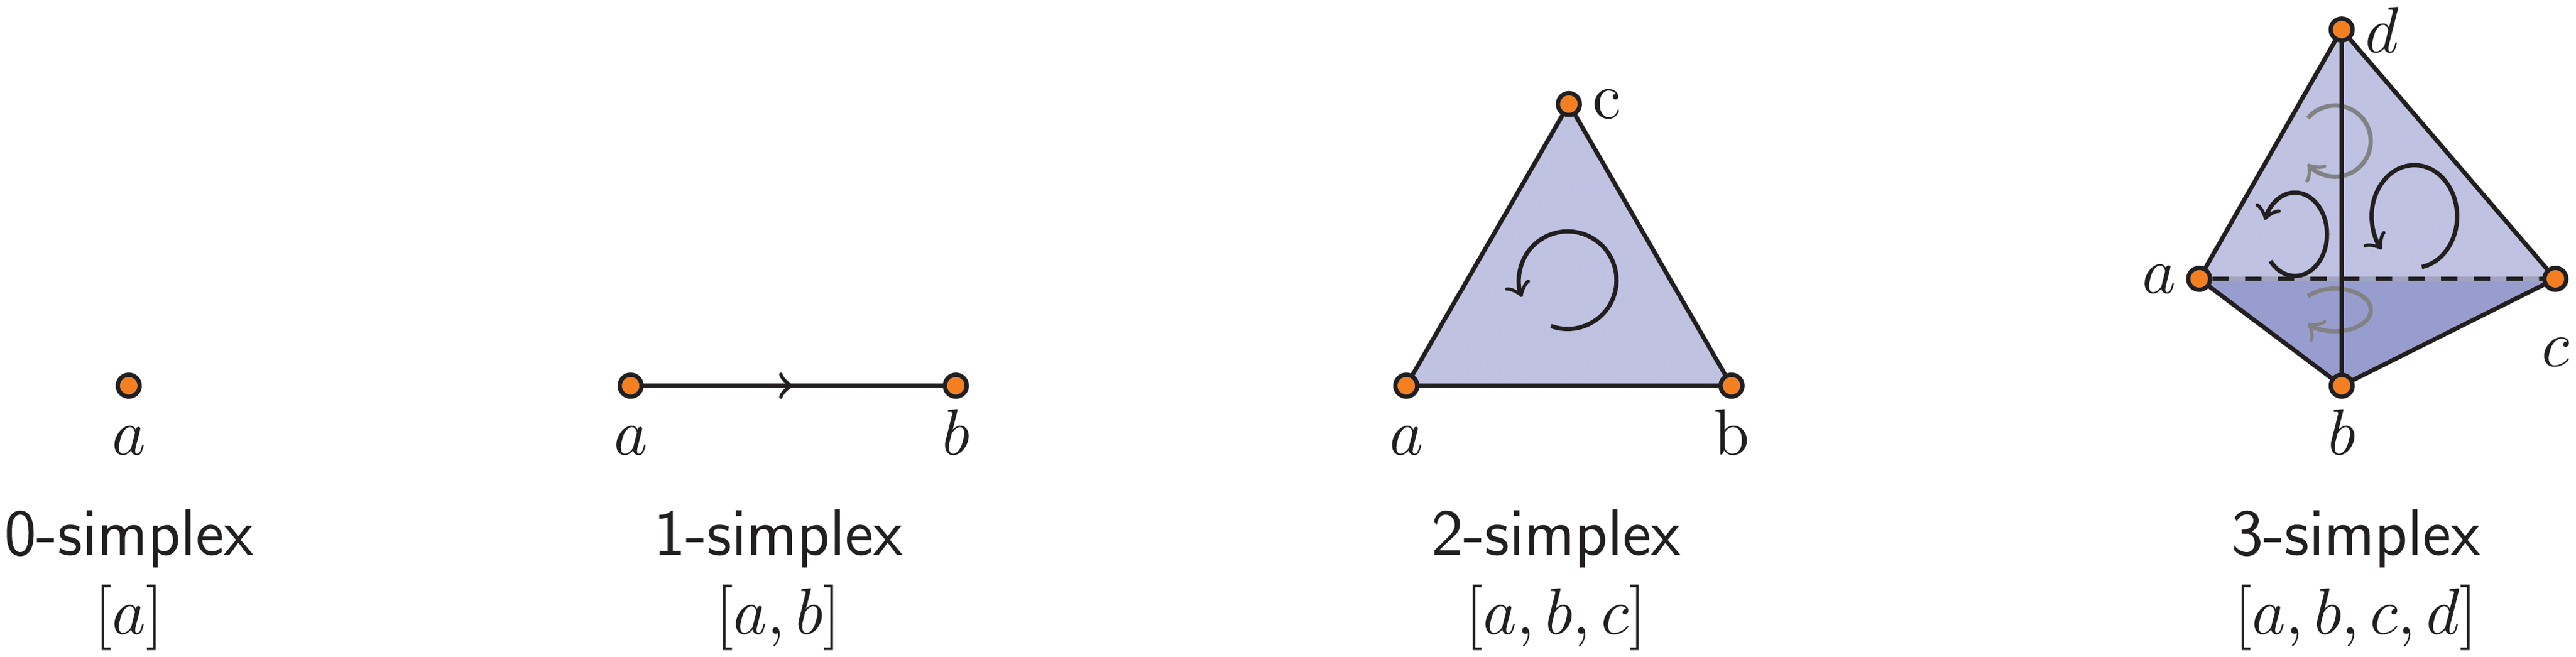
\includegraphics[scale = 0.65]{Orientacja.png}
\end{center}

\end{frame}

\begin{frame}{Orientacja 2}
\begin{itemize}
	\item Niestety orientację wierzchołka albo czworościanu ciężej sobie wyobrazić, będziemy więc musieli radzić sobie symbolicznie.
	\item Ponieważ są tylko dwie orientacje, to zmianę orientacji możemy reprezentować za pomocą znaku $-$, a zatem $ab = -ba$.
	\item Jeżeli zmienimy kolejność wierzchołków w naszym zorientowanym simpleksie, to orientacja ulega zmianie, a zatem $abc = -bac = bca = -cba = cab = -acb$.
\end{itemize}
\end{frame}

\begin{frame}{Łańcuchy}

\begin{itemize}
	\item Łańcuch to formalna suma simpleksów tego samego wymiaru (czyli dodawanie nic nie robi, po prostu jest).
	\item Przykład 1: $ab + bc + ca$ to łańcuch zrobiony z trzech boków trójkąta, czyli trójkąt ''pusty w środku''.
	\item Przykład 2: $a + b + c$ to łańcuch zrobiony z wierzchołków trójkąta. 
	\item Łańcuchy simpleksów o wymiarze $k$ tworzą grupę $C_k$. Element neutralny to pusty łańcuch (nic w nim nie ma), działanie to formalne dodawanie, a branie elementu odwrotnego to zmiana orientacji każdego simpleksu w łańcuchu.
\end{itemize}

\end{frame}

\begin{frame}{Brzegi i cykle}

\begin{itemize}
	\item Operator $\partial_k : C_k \to C_{k - 1}$ przypisuje łańcuchowi jego brzeg.
	\item Przykład: $\partial abc = bc - ac + ab = ab + bc + ca$, czyli brzegiem pełnego w środku trójkąta jest pusty w środku trójkąt.
	\item Cykl to łańcuch, który nie ma brzegu.
	\item Przykład: $ab + bc + ca$ to cykl, bo $\partial (ab + bc + ca) = (b - a) + (c - b) + (a - c) = 0$.
	\item Fakt: $\partial_k \partial_{k + 1} \sigma = 0$, czyli brzegi nie mają brzegów. Wobec tego brzegi są cyklami.
	\item Jeżeli dodamy simpleksy o przeciwnej orientacji, to się skrócą. Dzięki temu możemy rozkładać cykle na prostsze cykle.
\end{itemize}

\begin{center}
	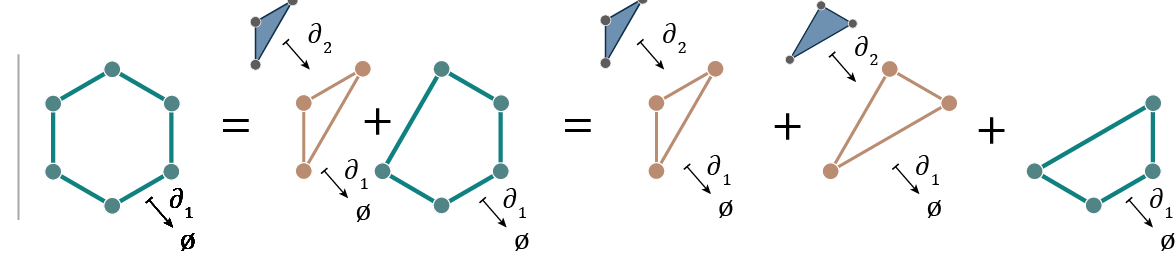
\includegraphics{Cykle.png}
\end{center}

\end{frame}

\begin{frame}{Grupy homologii}
\begin{itemize}
	\item $k$-tą grupę homologii kompleksu $C$ możemy zdefiniować tak: $H_k(C) = \text{ker}\ \partial_k / \text{im}\ \partial_{k + 1}$
	\item $\text{ker}\ \partial_k$ to grupa $k$-łańcuchów, które nie mają brzegu, czyli grupa $k$-cykli.
	\item $\text{im}\ \partial_{k + 1}$ to grupa $k$-łańcuchów, które są wynikiem działania $\partial_{k + 1}$ na $(k + 1)$-łańcuchach, czyli grupa $k$-brzegów.
	\item Mówiąc po ludzku: $k$-ta grupa homologii kompleksu $C$ to grupa $k$-cykli, ktore nie są $k$-brzegami.
	\item Po co nam było to wszystko? Otóż jeżeli cykl nie jest brzegiem, to znaczy, że okrąża on jakąś dziurę. Wobec tego $H_k(C)$ opisuje wszystkie sposoby, na jakie możemy w kompleksie $C$ chodzić dookoła $k$-wymiarowych dziur.
\end{itemize}
\end{frame}

\begin{frame}{Grupy homologii -- przykład 1}

\begin{center}
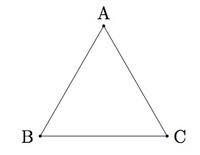
\includegraphics[scale = 0.7]{Triangle.jpeg}
\end{center}

\begin{itemize}
	\item Każdy wierzchołek jest $0$-cyklem, bo nie ma brzegu. Stąd $\text{ker}\ \partial_0 = \mathbb{Z}^3$ (każdy cykl jest zrobiony z kombinacji wierzchołków).
	\item Z drugiej strony mamy $\partial_1 ab = b - a$, $\partial_1 bc = c - b$, $\partial_1 ca = a - c$. Widać, że $\partial_1 ca = -(\partial_1 ab + \partial_1 bc)$, a zatem są tylko dwa niezależne brzegi i stąd $\text{im}\ \partial_1 = \mathbb{Z}^2$.
	\item Wobec tego $H_0(abc) = \mathbb{Z}^3 / \mathbb{Z}^2 = \mathbb{Z}$.
\end{itemize}

\end{frame}

\begin{frame}{Grupy homologii -- przykład 2}

\begin{center}
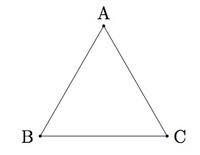
\includegraphics[scale = 0.7]{Triangle.jpeg}
\end{center}

\begin{itemize}
	\item Jest tylko jeden $1$-cykl, mianowicie $ab + bc + ca$, gdyż $\partial_1 (ab + bc + ca) = (b - a) + (c - b) + (a - c) = 0$. Stąd $\text{ker}\ \partial_1 = \mathbb{Z}$.
	\item Z drugiej strony mamy $\text{im}\ \partial_2 = 1$ (grupa trywialna), gdyż żaden $1$-łańcuch nie jest brzegiem żadnego $2$-simpleksu, czyli trójkąta. Wynika to z faktu, że na obrazku nie ma trójkąta (przypominam, że trójkąt jest pełny w środku).
	\item Wobec tego $H_1(abc) = \mathbb{Z} / 1 = \mathbb{Z}$.
	\item Wyższe grupy homologii są trywialne, gdyż nie ma żadnych $k$-cykli dla $k \geq 2$.
\end{itemize}

\end{frame}

\begin{frame}{Grupy homologii -- interpretacja przykładu}
\begin{itemize}
	\item Jak zinterpretować powyższe wyniki? Gdzie są nasze dziury?
	\item Dla $H_1$ sprawa jest prosta -- jest jedna dziura, którą można chodzić $k$ razy zgodnie z ruchem wskazówek zegara ($+k$), $k$ razy przeciwnie do ruchu wskazówek zegara ($-k$), albo w ogóle nigdzie nie iść ($0$). Grupa takiego chodzenia dookoła dziury jest więc izomorficzna z $\mathbb{Z}$, czyli dokładnie tak, jak nam wyszło.
	\item Dla $H_0$ z wyobraźnią jest trudniej. Wystarczy nam zatem wiedzieć jedynie, że $H_0(C)$ reprezentuje ilość spójnych składowych kompleksu $C$.	
\end{itemize}
\end{frame}

\begin{frame}{Liczby Bettiego}
\begin{itemize}
	\item Grupy homologii byłyby dość upierdliwe do zaimplementowania w większości mainstreamowych języków programowania.
	\item Nie mówiąc o tym, że w przykładzie ciągle pojawiała się grupa $\mathbb{Z}$ i nie był to przypadek -- przydałaby się jakaś prostsza reprezentacja dziur.
	\item Wobec tego definiujemy liczby Bettiego: dla kompleksu $C$ mamy $\beta_k(C) = \text{rank}(H_k(C))$.
	\item Po ludzku: $k$-ta liczba Bettiego to liczba generatorów $k$-tej grupy homologii.
	\item Intuicja: $\beta_0$ to liczba spójnych składowych, $\beta_1$ to liczba dziur jednowymiarowych, $\beta_2$ to liczba dziur dwuwymiarowych etc.
\end{itemize}
\end{frame}

\begin{frame}{Liczby Bettiego -- przykład 1}

\begin{center}
	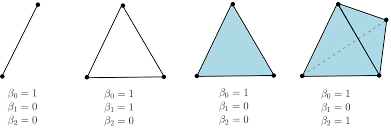
\includegraphics[scale = 0.7]{LiczbyBettiego.png}
\end{center}

\begin{itemize}
	\item Odcinek jest spójny ($\beta_0 = 1$) i nie ma dziur ($\beta_k = 0, k \geq 1$).
	\item Pusty trójkąt jest spójny ($\beta_0 = 1$) i ma jednowymiarową dziurę ($\beta_1 = 1$), ale nie ma więcejwymiarowych dziur ($\beta_k = 0, k \geq 2$).
	\item Pełny trójkąt jest spójny ($\beta_0 = 1$) i nie ma dziur ($\beta_k = 0, k \geq 1$).
	\item Pusty czworościan (czyli same ściany, bez wnętrza) jest spójny ($\beta_0 = 1$), nie ma $1$-wymiarowych dziur ($\beta_1 = 0$), ma $2$-wymiariową dziurę ($\beta_2 = 1$) i nie ma więcejwymiariowych dziur ($\beta_k = 0, \geq 3$).
\end{itemize}

\end{frame}

\begin{frame}{Liczby Bettiego -- przykład 2}

\begin{center}
	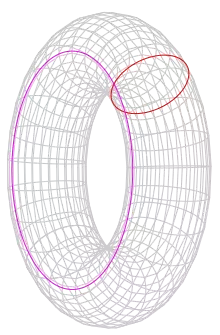
\includegraphics[scale = 1.5]{GrupyHomologiiTorusa.png}
\end{center}

Liczby Bettiego dla torusa: $(\beta_0, \beta_1, \beta_2) = (1, 2, 1)$ i $\beta_k = 0$ dla $k \geq 3$. Jest tak dlatego, że torus jest spójny ($\beta_0 = 1$), ma dwie niezależne od siebie jednowymiarowe dziury ($\beta_1 = 2$; zaznaczone na rysunku -- nie da się w sposób ciągły przekształcić jednej w drugą) oraz jedną dwuwymiarową dziurę ($\beta_2 = 1$; pamiętajmy, że torus jest pusty w środku).
	
\end{frame}
	
\begin{frame}{Liczby Bettiego -- ćwiczenia}

Ile wynoszą liczby Bettiego dla:

\begin{itemize}
	\item Zbiorów punktów?
	\item Grafów?
	\item Simpleksów?
	\item Brzegów simpleksów?
	\item $k$-wymiarowych sześcianów?
	\item Brzegów $k$-wymiarowych sześcianów?
\end{itemize}

\end{frame}

\begin{frame}{Liczby Bettiego -- podsumowanie}
\begin{itemize}
	\item Ponieważ w $n$-wymiarowej przestrzeni nie może być $\geq n$-wymiarowych dziur, to liczby Bettiego wynoszą zero dla $k \geq$ wymiar przestrzeni.
	\item Dzięki temu możemy opisać przybliżony kształt przestrzeni za pomocą niezbyt długiego ciągu liczb.
	\item Fajnie, ale jak technicznie znaleźć ten przybliżony kształt danych?
\end{itemize}
\end{frame}

\section{Topologiczna Analiza Danych}

\begin{frame}{Dopasowywanie kompleksu do danych 1}
\begin{itemize}
	\item Załóżmy, że mamy $N$ punktów danych pochodzących z $k$-wymiarowej przestrzeni $X$ (nie musi być $X = \mathbb{R}^k$, ale zazwyczaj pewnie tak będzie).
	\item Żeby teoria homologii poszła w ruch, musimy dopasować do danych jakiś kompleks.
	\item Jeżeli nam się to uda, to będziemy mogli opisać jego przybliżony kształt (czyli strukturę dziur) za pomocą liczb Bettiego.
	\item Ponieważ chmura $N$ punktów daje co najwyżej $N$-wymiarowy kompleks, to do opisu kształu danych wystarczy $\text{min}(N, k)$ liczb.
	\item Jeżeli $N$ i $k$ są bardzo duże to możemy mieć problem, ale spodziewamy się, że najciekawsze i tak będzie niskowymiarowe przybliżenie naszego kształtu, więc nie musimy się przejmować.
\end{itemize}
\end{frame}

\begin{frame}{Dopasowywanie kompleksu do danych 2}
\begin{itemize}
	\item Potrzebna będzie nam metryka $d: X \times X \to \mathbb{R}$.
	\item Pomysł na dopasowanie kompleksu jest następujący.
	\item Wybieramy pewien $\varepsilon \in \mathbb{R}$. Jeżeli mamy $n$ punktów, które leżą w odległości $\leq 2\varepsilon$ każdy od każdego, to wrzucamy do naszego kompleksu odpowiadający im $n$-simpleks.
	\item Pytanie: jaki $\varepsilon$ wybrać?
	\item Jeżeli nie wiesz jaki wybrać parametr, wybierz wszystkie: \url{https://sauln.github.io/blog/nerve-playground/}
\end{itemize}
\end{frame}

\begin{frame}{Kształty w różnej skali}
\begin{itemize}
	\item Parametr $\varepsilon$ możemy rozumieć jako skalę w której przyglądamy się naszym danym.
	\item Jeżeli $\varepsilon$ jest bardzo małe, to widzimy gołe punkty bez żadnych powiązań.
	\item Jeżeli $\varepsilon$ jest bardzo duże, to widzimy jeden wielgachny punkt bez żadnej wewnętrznej struktury.
	\item Dla pośrednich $\varepsilon$ jesteśmy w stanie dostrzec różne ciekawe kształty.
	\item Każdy z tych kształtów powstaje w pewnej skali, a w miarę jak zwiększamy skalę, znika i staje się częścią jakiegoś większego kształtu.
\end{itemize}
\end{frame}

\begin{frame}{Homologia persystentna}
\begin{itemize}
	\item Taka jest właśnie idea stojącą za teorią (techniką?) homologii persystentnej.
	\item Żeby dowiedzieć się czegoś o danych, sprawdzamy w jakiej skali rodzą się, a w jakiej umierają dziury różnego wymiaru.
	\item Im dłużej dana dziura żyje, tym lepiej oddaje ona prawdziwy kształt danych. Dziury żyjące krótko są jedynie przejawem szumu.
\end{itemize}
\end{frame}

\begin{frame}{Topologiczna analiza danych -- podsumowanie}
\begin{itemize}
	\item Na początku postawiliśmy sobie za cel znajdowanie kształtu danych i udało nam się zapoznać z podstawowymi ideami, które to umożliwiają.
	\item Pozostaje jeszcze kwestia tego, jak wypada to wszystko w praktyce -- algorytmy, wyniki etc.
	\item Niestety 15 minut to za krótko, żeby opowiedzieć od podstaw do praktyki o tak skomplikowanym zagadnieniu jak topologiczna analiza danych.
	\item Jeżeli chcesz dowiedzieć się więcej, musisz zbadać temat samemu.
	\item Mam nadzieję, że dzięki tej prezentacji twoje poszukiwania będą mniej bolesne niż moje.
\end{itemize}
\end{frame}

\begin{frame}{Przydatne materiały do czytania}
\begin{itemize}
	\item Krótkie wprowadzenie do topologicznej analizy danych: \url{https://jsseely.github.io/notes/TDA/}
	\item Polecam dokładnie je przejrzeć: zawiera linki do notatek wprowadzających do topologii, filmików ilustrujących homologię persystentną w nieco bardziej interaktywny sposób, prac naukowych z wynikami oraz listy oprogramowania, w tym do niewspomnianego podczas prezentacji algorytmu Mapper.
\end{itemize}
\end{frame}

\begin{frame}{Przydatne materiały do oglądania}
\begin{itemize}
	\item O simpleksach, kompleksach i triangulacji: \url{https://www.youtube.com/watch?v=9vLAZkOk3IA}
	\item Polecam obejrzeć wszystkie filmiki z powyższej serii, stanowią wprowadzenie do homologii persystentnej o niebo bardziej interaktywne niż niniejsza prezentacja.
	\item Głównie o algorytmie Mapper: \url{https://www.youtube.com/watch?v=x3Hl85OBuc0}
	\item O Pythonowych narzędziach do topologii: \url{https://www.youtube.com/watch?v=AWoeBzJd7uQ}
\end{itemize}
\end{frame}
	
\end{document}
